\documentclass[a4paper, 11pt]{article}

\usepackage[left=1.5cm, right=1.5cm, top=2cm, bottom=2cm]{geometry}

\usepackage[utf8]{inputenc} 
\usepackage[T1]{fontenc}      
\usepackage[french,english]{babel}  
\usepackage{lmodern}

\usepackage{amsmath, mathtools}
\usepackage{amssymb}
\usepackage{amsthm}
\usepackage{empheq}

\usepackage{graphicx,wrapfig}
\usepackage{subfig}

\usepackage{listings}
\usepackage{color} %red, green, blue, yellow, cyan, magenta, black, white
\definecolor{mygreen}{RGB}{28,172,0} % color values Red, Green, Blue
\definecolor{mylilas}{RGB}{170,55,241}

\graphicspath{{../figures/}}
\usepackage{caption}

\begin{document}
\title{Rendu DM3 Modèles probabilistes graphiques} 
\author{Yoann Pradat}
\maketitle

\paragraph{Exercise 1}

\textbf{1.1} The HMM model we are considering has chain $(q_t)_{t=1,\dots,T}$ and observations $(u_t)_{t=1,\dots,T}$.
Each node of the chain can take $K=4$ different states. We will note $\pi = (\pi_1, \dots, \pi_K)$ the distribution of
the first node of the chain $q_1$. In the class the formulas for the $\alpha$ and $\beta$ recursions are given as
functions of the potentials $\psi$. Let's define them in our model. 
\begin{equation*}
  \frac{1}{Z}\psi_{q_1}(q_1) = \pi_{q_1}, \quad \psi_{q_{t-1}, q_t}(q_{t-1}, q_t) = a_{q_{t-1}, q_t}, \quad \psi_{q_t,
  u_t}(q_t,u_t) = \frac{(\text{det} \Sigma_{q_t})^{-\frac{1}{2}}}{2\pi} e^{-\frac{1}{2}(u-\mu_{q_t})^T\Sigma_{q_t}^{-1}(u-\mu_{q_t})}
\end{equation*}

\textbf{1.2} Let $n$ be the iteration we are at in the EM algorithm. The complete log-likelihood 
for the data $(u_t)_{t=1,\dots,T}$ with states $(q_t)_{t=1,\dots,T}$ for the parameters $\theta_{n-1} = (\pi, a, \mu, \Sigma)$  is
\small\begin{equation*}
  l_c(\theta) = \sum_{k=1}^K \delta_{q_1{=}k} \log(\pi_k) + \sum_{t=2}^T \sum_{k,l=1}^K \delta_{q_{t-1}{=}k, q_t{=}l} \log (a_{k,l}) + 
  \sum_{t=1}^T \sum_{k=1}^K  \delta_{q_t{=}k} \log \mathcal{N}(u_t | \mu_k, \Sigma_k)
\end{equation*}\normalsize

Realizing the $E$ step is done by replace indicators $\delta$ with conditional distributions hence the following quantity
to be maximized with respect to $\theta$ in the $M$ step.
\small\begin{equation*}
  \mathcal{L}_{\theta} = \sum_{k=1}^K p_{\theta_{n-1}}(q_1{=}k|u_{1\dots T}) \log(\pi_k) + \sum_{t=2}^T \sum_{k,l=1}^K p(q_{t-1}{=}k, q_{t}{=}l|u_{1\dots T}) 
  \log (a_{k,l}) + \sum_{t=1}^T \sum_{k=1}^K  p_{\theta_{n-1}}(q_t{=}k|u_{1\dots T})   \log \mathcal{N}(u_t | \mu_k, \Sigma_k)
\end{equation*}\normalsize

We deduce the following updates of the parameters $\theta$ in the M step at $n^{th}$ iteration
\small\begin{equation*}
  \boxed{\widehat{\pi_k} = \frac{p_{n-1}(1, k)}{\sum_{l=1}^K p_{n-1}(1,l)} \qquad \widehat{a_{k,l}} =
    \frac{\sum_{t=2}^T p_{n-1}(t,k,l)}{\sum_{t=2}^T p_{n-1}(t,k)} \qquad \hat{\mu_k} = \frac{\sum_{t=1}^T p_{n-1}(t,k)
  u_t}{\sum_{t=1}^T p_{n-1}(t,k)} \qquad \hat{\Sigma_k} = \frac{\sum_{t=1}^T p_{n-1}(t,k) (u_t - \mu_k)(u_t - \mu_k)^T}{\sum_{t=1}^T p_{n-1}(t,k)}}
\end{equation*}\normalsize

where $p_{n-1}(t,k) =  p_{\theta_{n-1}}(q_t{=}k|u_{1\dots T})$, $p_{n-1}(t,k,l) =  p_{\theta_{n-1}}(q_{t-1}{=}k,
q_t{=}l|u_{1\dots T})$. The calculation of conditional distributions in the formulas have been implemented in question
\textbf{1.1}.

\begin{figure}[!h]
  \hspace*{\fill}%
  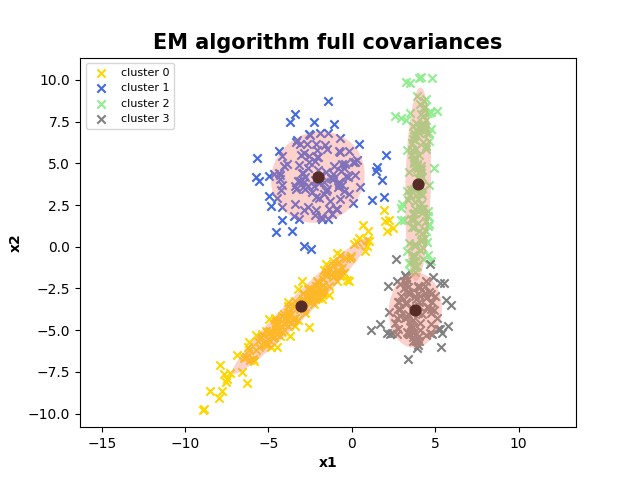
\includegraphics[width=7cm]{em_full.png}\hfill%
  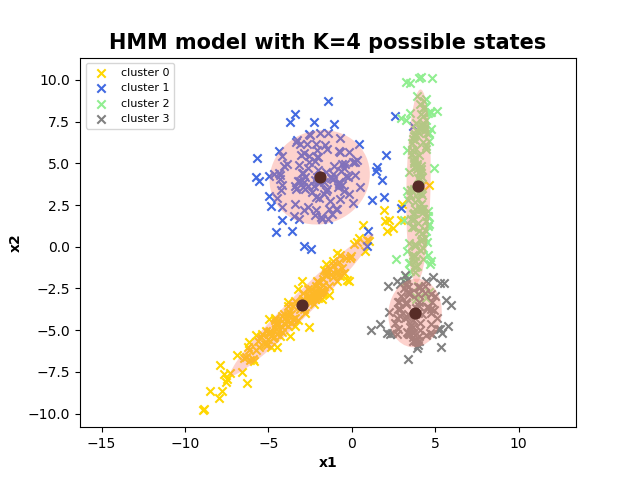
\includegraphics[width=7cm]{hmm.png}%
  \hspace*{\fill}%
  \label{fig:comparison}
\end{figure}

\textbf{1.5} We see that contrary to GMM model, HMM model may assign a point to a cluster whose center is not the
closest (whatever the distance on $\mathbb{R}^2$). However the overall fit with HMM is better as the complete log-likelihood is lower both on 
the train set (-1,555.92 vs -2,345.97) and the test set (-1,636.79 vs -2,425.99). We also see that the parameters $\mu$ and $\Sigma$ learned by
GMM and HMM models are very similar.
\end{document}



